% Chapter 3: Model
\chapter{Model}

\section{Model Architecture}
ใช้ DistilBERT ซึ่งเป็น Pre-trained transformer model ด้วยเทคนิค distillation เป็นโมเดลที่มีขนาดเล็ก แต่ยังคงประสิทธิภาพส่วนใหญ่ไว้อยู่ \cite{victor2019distilbert} เนื่องจากข้อมูลมีจำนวนน้อย การ fine-tune โมเดลที่มีปริมาณ parameter น้อยจะสามารถทำได้ง่ายกว่า

สถาปัตยกรรมโมเดลประกอบด้วย pre-trained DistilBERT ตามด้วย fully connected layer ที่ใช้ sigmoid เป็น activation function ที่จะทำหน้าที่แปลง output embeddings เป็นคะแนนความน่าจะเป็นของแต่ละคลาสทั้ง 18 คลาส

\section{Training Configuration}
\begin{itemize}
    \item Optimizer: AdamW, learning rate 2e-5
    \item Loss function: BCEWithLogitsLoss, pos\_weight
    \item Batch size: 16
    \item Max length: 512
    \item Number of epochs: 30
\end{itemize}
\clearpage

\begin{figure}[ht]
    \centering
    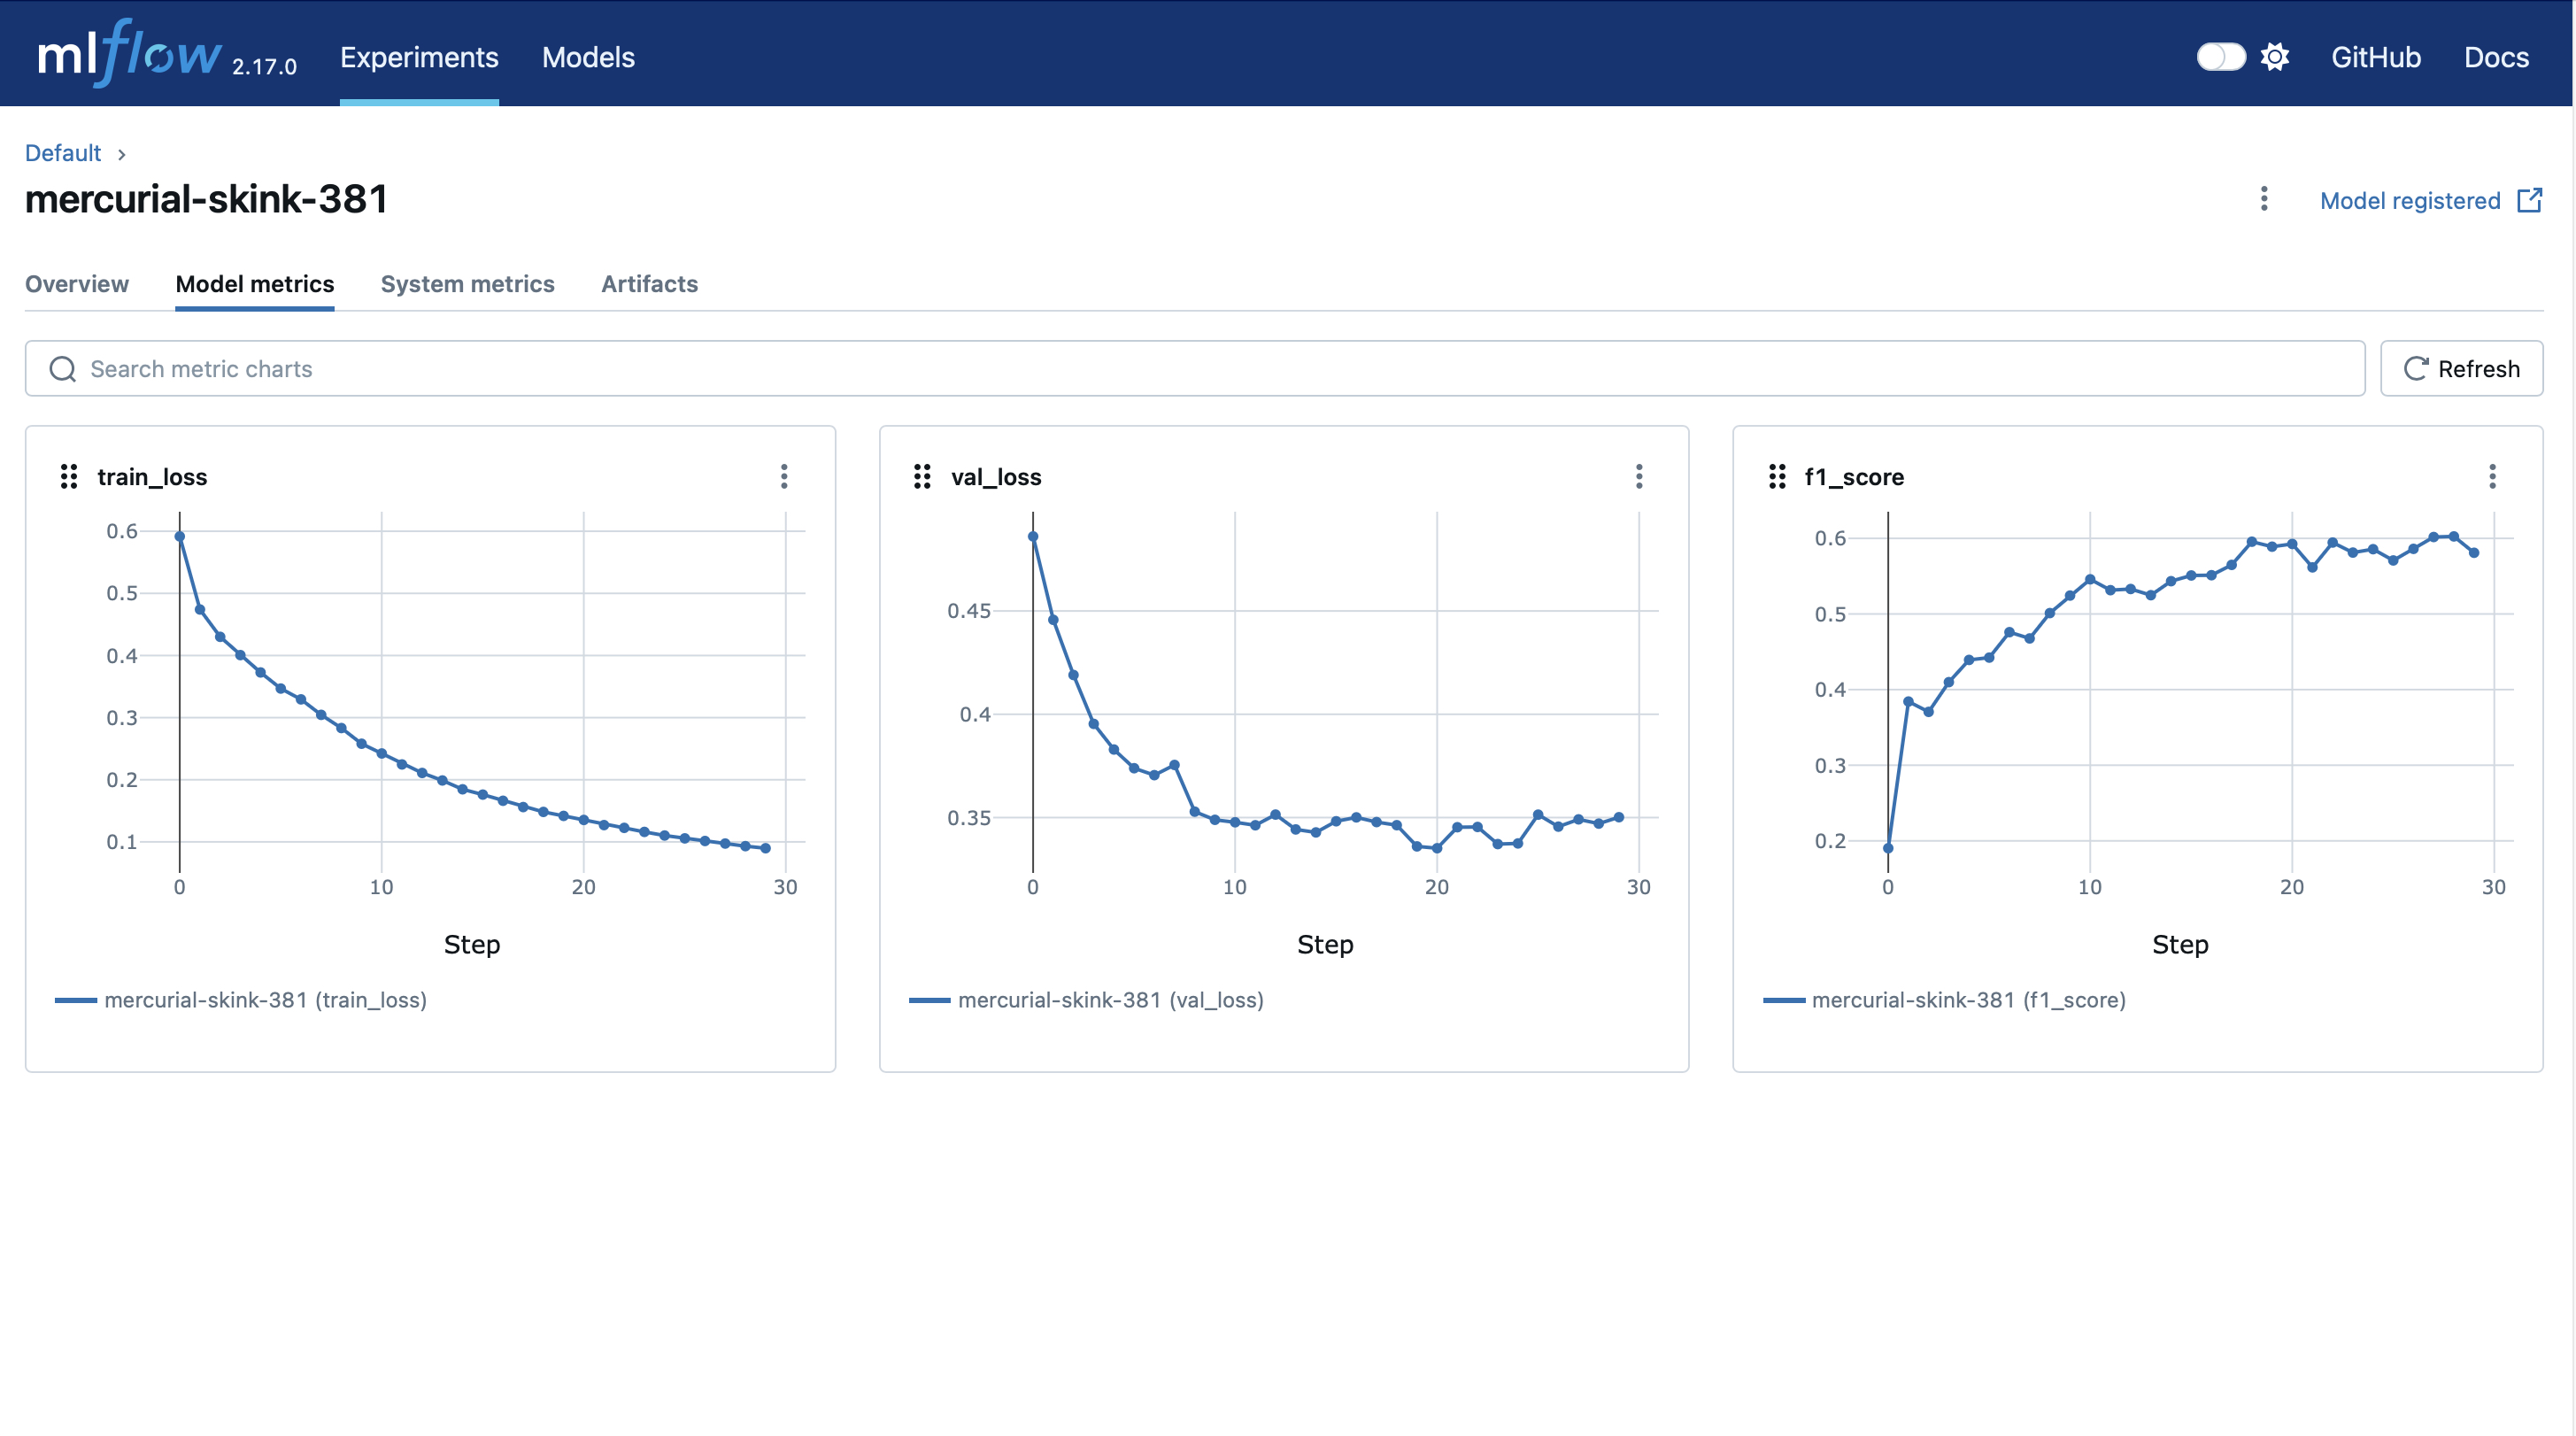
\includegraphics[width=\imgwidth]
    {images/model_training_graph.jpg}
    \caption{Model training graph}
    \label{fig:model_training_graph}
\end{figure}

\begin{figure}[ht]
    \centering
    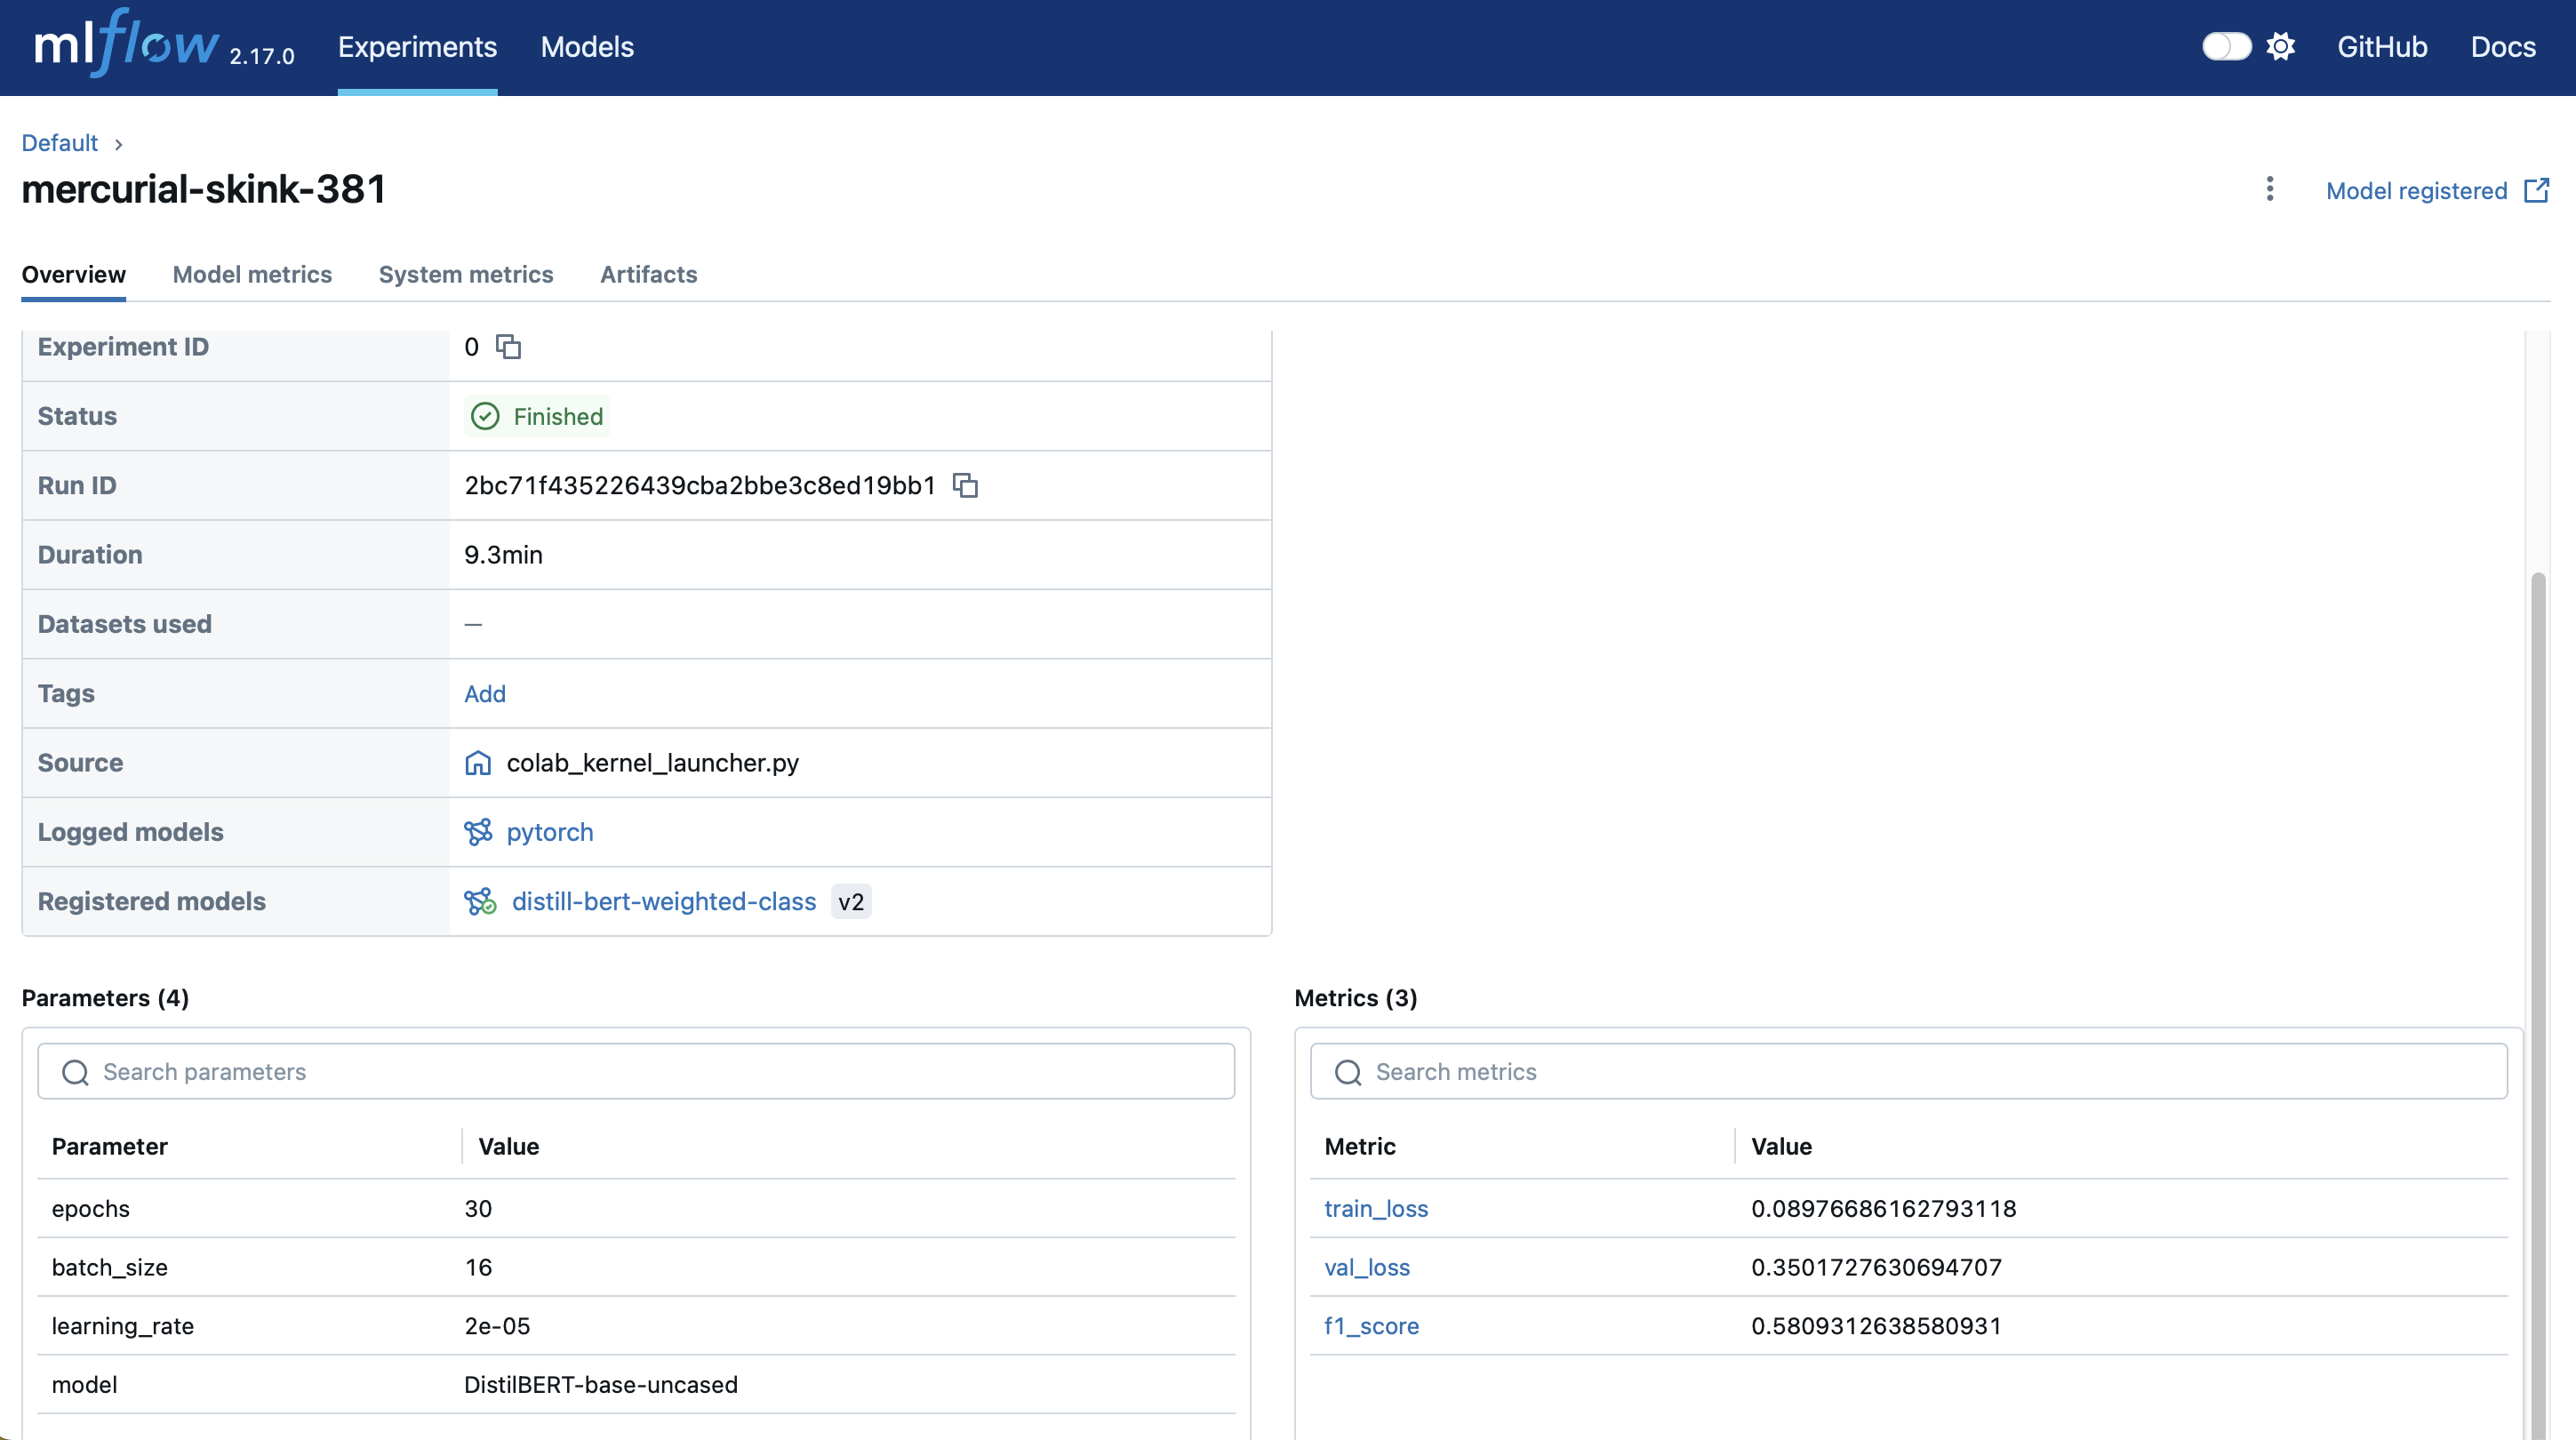
\includegraphics[width=\imgwidth]
    {images/model_metrics.jpg}
    \caption{Model metrics from MLflow}
    \label{fig:model_metrics.jpg}
\end{figure}

โมเดลมี F1 Validation อยู่ที่ 0.5809 และค่า val\_loss เริ่มลู่เข้าที่ Epoch 10